\documentclass{article}
\usepackage[utf8]{inputenc}
\usepackage{amsmath}
\usepackage{amssymb}
\usepackage[right=3.5cm, left=3.5cm, top=3.5cm, bottom=3.5cm]{geometry}
\usepackage{graphicx}
\usepackage{hyperref}

\title{\textbf{The Fast Bilateral Solver}
\\
\textsc{Numerical imaging - Project report}}
\author{Guillaume Dalle, MVA 2018-2019}
\date{}

\begin{document}

\maketitle

\tableofcontents

\newpage

\section{Algorithm description}

Filtering is one of the most fundamental building blocks of image processing. The simplest smoothing method is a Gaussian filter, averaging pixels that are close together in a geometric sense. However, such a filter doesn't differentiate between smooth areas and sharp edges, which become blurred in the process.

\medskip

This project is based on "The Fast Bilateral Solver", by Jonathan T. Barron \& Ben Poole \cite{barron_fast_2016}.
The goal of the article is to define and efficiently implement an edge-aware smoother. This technology has countless applications, ranging from simple image "cartooning" or sharpening to automatic colorization or segmentation.

\subsection{The model}

In this section, we introduce the problem we want to solve. In simple terms, given a reference image and a target image, we want to produce a new result that is chromatically similar to the target image while respecting the structure (including edges) of the reference image.

For instance, in a colorization task:
\begin{itemize}
    \item the reference image will be the original black and white image (because we want the coloring to respect geometric proximity and stop at edges)
    \item the target image will be the color channels of a user-marked black and white image (giving us a clue of the real colors in certain locations)
\end{itemize}

\subsubsection{A high-dimensional optimization problem}

From now on, we will work with a reference image $\textbf{p} = (p_i)_{i \in [N]}$ made of pixels with several channels, e.g. in the  LUV space (luminance - chrominance). To avoid the trap of purely geometric filtering, we will consider the position $p_i \in \textbf{R}^5$ of pixel $i$ as being the concatenation of:
\begin{itemize}
    \item its geometric coordinates $(p_i^x, p_i^y) \in [0, x_{max}] \times [0, y_{max}]$
    \item its channel intensities, e.g. $(p_i^l, p_i^u, p_i^v) \in [0, 255]^3$ in the LUV case
\end{itemize}

This combination idea was first introduced by \cite{tomasi_bilateral_1998}, among others.

With this in mind, we can define an edge-aware measure of similarity between two pixels of the reference image, taking into account not only their spatial proximity but also their color proximity. Given a vector $\sigma = (\sigma_{xy}, \sigma_l, \sigma_{uv})$ of standard deviations, we define a gaussian similarity between pixels $i$ and $j$ in the following way:
\begin{equation}
    W_{i, j} = \exp \left(
    - \frac{|| (p_i^x, p_i^y) - (p_j^x, p_j^y) ||^2}{2 \sigma_{xy}^2}
    - \frac{| p_i^l - p_j^l |^2}{2 \sigma_l^2}
    - \frac{|| (p_i^u, p_i^v) - (p_j^u, p_j^v) ||^2}{2 \sigma_{uv}^2}
     \right)
\end{equation}

Suppose now that we want to build another image $\textbf{x} = (x_i)_{i \in [N]}$ with the same shape as $\textbf{p}$ but just one channel, that is $x_i \in [0, 255]$ (the multi-channel case is an easy generalization).

We wish this new image to be both:
\begin{enumerate}
    \item Smooth with respect to the edge-aware similarity between pixels of the reference image $\textbf{p}$.
    \item Close to a target image $\textbf{t}$ in terms of channel values.
\end{enumerate}

This translates into the following optimization problem:
\begin{equation} \label{optim}
    \min_{x \in \textbf{R}^N} \frac{\lambda}{2} \sum_{1 \leq i, j \leq N}{\hat{W}_{i, j} (x_i - x_j)^2} + \sum_{1 \leq i \leq N}{c_i (x_i - t_i)^2}
\end{equation}

Here $t_i$ is the target value of pixel $i$, $c_i$ expresses the confidence we have in the value of that target. $\lambda$ defines the balance between both objectives of this minimization.
Finally, $\hat{W}$ is a bistochastized version of $W$, which is meant to improve smoothing performance (for instance by ensuring conservation of the mean).

\medskip

Unfortunately, this optimization problem is not tractable, since $N = x_{max} \cdot y_{max}$ is usually very large (a few millions). We therefore have to find an approximation that enables us to solve it in reasonable time.

\subsubsection{Splat-blur-slice and the bilateral space}

This is where the bilateral space comes in. The main idea, described in \cite{barron_fast_2015}, is to go from a huge set of pixels to a smaller set of "vertices" that approximate them. 

\medskip

Essentially, we can view a LUV image $\textbf{p}$ as a set of points in a a 5-dimensional space of positions $p = (p^x, p^y, p^l, p^u, p^v)$. To make coordinates homogeneous, we first scale them by their respective standard deviations $\sigma$. We then approximate the scaled positions with a periodic lattice, assigning each pixel to one or more of its nearest neighbors.

The lattice points are called \textit{vertices}, and they live in the \textit{bilateral space}. The goal is that the number of vertices $V$ should be much smaller than the number of pixels $N$, and we will see that it is.

\medskip

Now imagine for a moment that we must filter a vector of pixel values $\textbf{x}$ with a simple matrix multiplication: forget about the optimization problem \eqref{optim}, we just want to compute $W\textbf{x}$.
To approximate that operation (which we deem too expensive to perform exactly), we use the bilateral space through the following three-step procedure:
\begin{enumerate}
    \item \textit{Splat}: Split each pixel value $x_i$ onto the vertices that are closest to $p_i$
    \item \textit{Blur}: Perform a smoothing operation of vertex values $y_v$ in the bilateral space
    \item \textit{Slice} : Interpolate the new value $\tilde{x}_i$ from the blurred values $\tilde{y}_v$ of the vertices closest to $p_i$
\end{enumerate}
This is represented graphically in figure \ref{fig:SBS}.

\begin{figure}
    \centering
    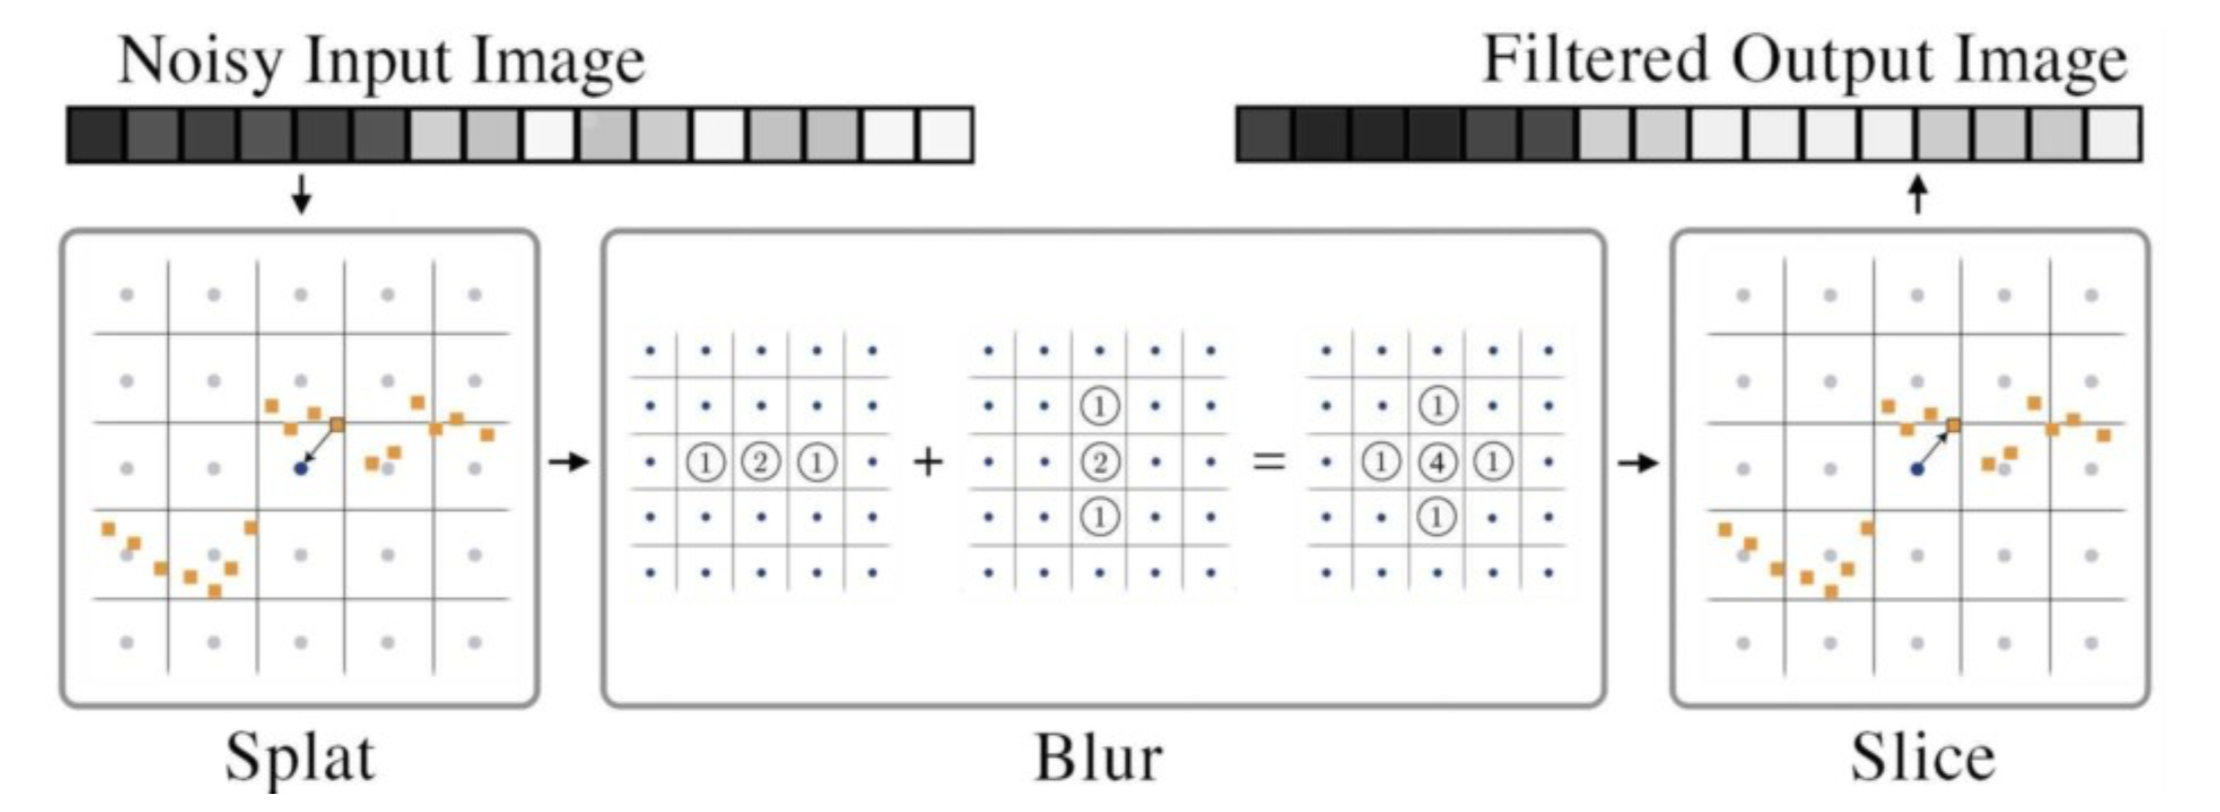
\includegraphics[width=\linewidth]{pictures/SBS.png}
    \caption{Illustration of the splat-blur-slice procedure on a 1D image (taken from \cite{barron_fast_2015})}
    \label{fig:SBS}
\end{figure}

\medskip

In the simplified bilateral grid (adapted by \cite{barron_fast_2015} from \cite{chen_real-time_2007}) which is the one we implemented, the lattice is composed of the integer points $\textbf{Z}^5$, and the blurring operation will simply average a vertex with its 2 closest neighbors on each of the 5 axes: this boils down to a sum of 5 $(1, 2, 1)$ filters along different directions.

We indeed observe a huge dimension reduction, because we are actually sampling from a 2D structure inside a 5D lattice. Indeed, only vertices that are close to the original image (a 2D manifold in $\textbf{R}^5$) will actually matter, so that we can discard the rest.

\medskip

A final remark is that contrary to standard gaussian filtering, the smoothing parameters do not affect the blurring operation per se, since the bilateral blur scheme (1, 2, 1) remains constant. Instead, $\sigma$ defines the scaling of the bilateral grid and therefore the precision of nearest neighbor assignment.

If for instance $\sigma_l$ is large, then lots of scaled positions $p / \sigma$ will have a nearest vertex with the same luminance, and therefore the smoothing radius on luminance will be very wide.

\subsubsection{A low-dimensional linear system}

Although the original articles introducing splat-blur-slice techniques did not see it that way, the example of matrix multiplication suggests that this procedure can be thought of as an approximate matrix factorization of $W$:
\begin{equation}
    W \simeq S^T B S
\end{equation}

This interpretation is illustrated in figure \ref{fig:SBS2}.

\begin{figure}
    \centering
    \hspace{0.3cm}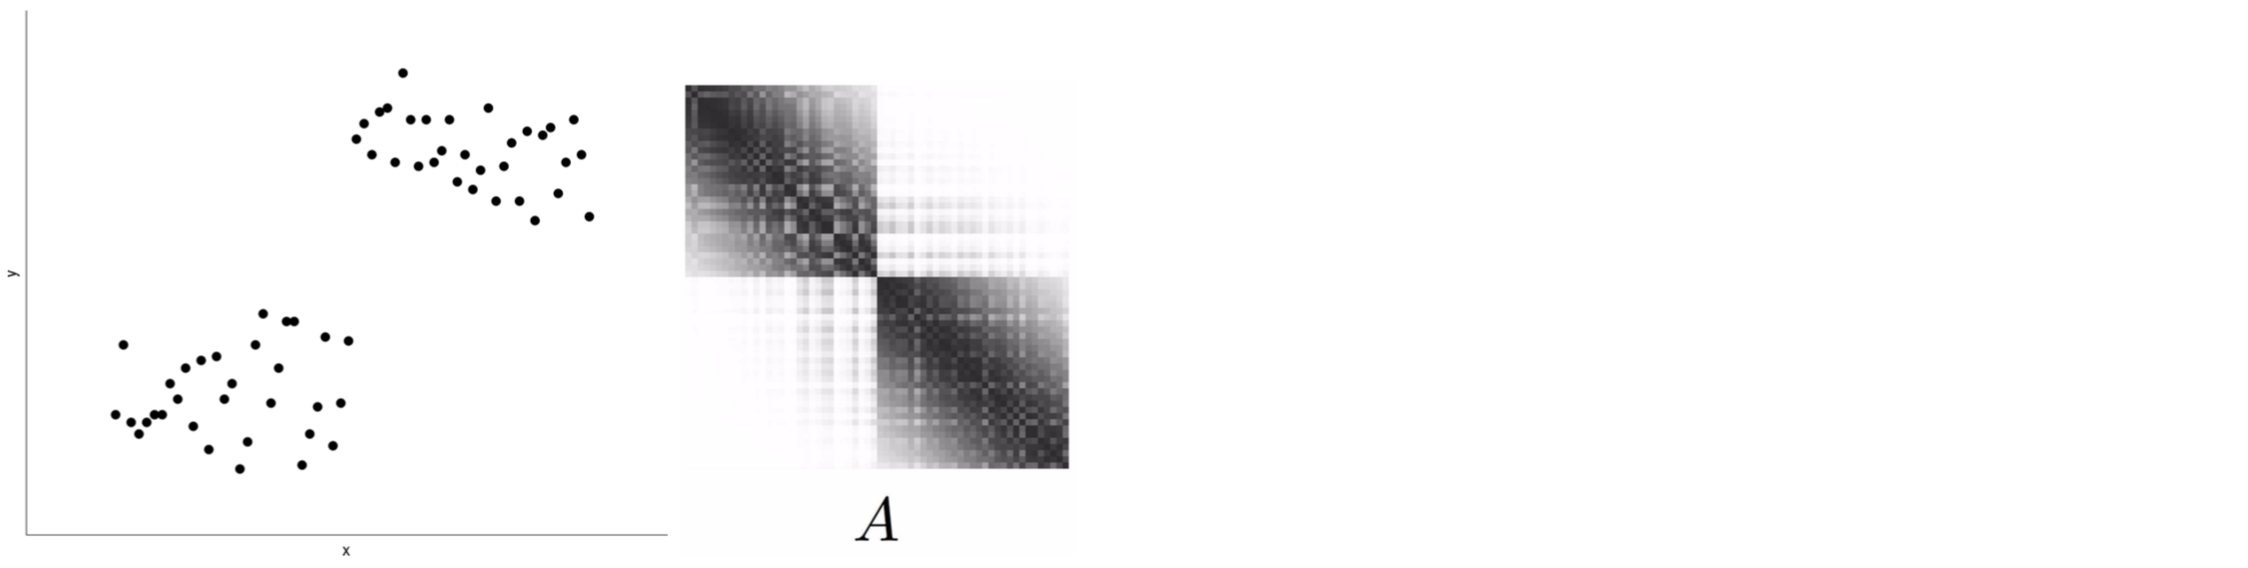
\includegraphics[width=14cm]{pictures/SBS2_0.png}
    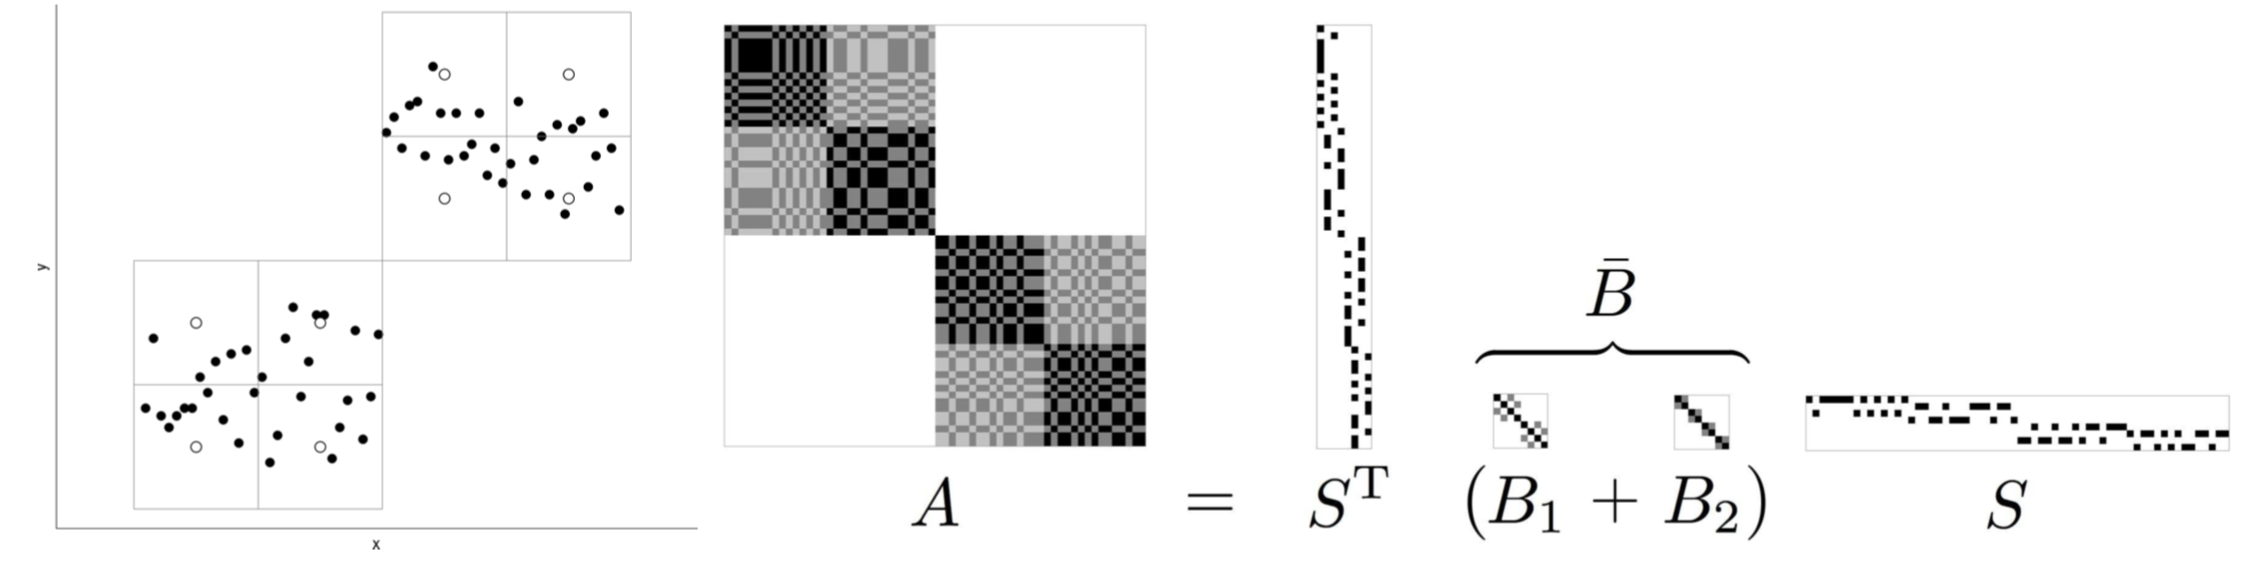
\includegraphics[width=14cm]{pictures/SBS2.png}
    \caption{Illustration of the splat-blur-slice factorization on a 1D image (taken from \cite{barron_fast_2015})}
    {\it \small The black dots are the pixel positions, the white dots are the vertices of the bilateral grid. The $x$-axis is the spatial position of the pixels/vertices, and the $y$-axis is the luminance position. The true matrix $W$ (here $A$) is shown above, and below is its splat-blur-slice approximation. The matrix $S$ links each pixel to one of the 8 bilateral vertices, and the matrix $B$ is the sum of two (1, 2, 1) blurs in the bilateral space: one along the $x$-axis and one along the $y$-axis.}
    \label{fig:SBS2}
\end{figure}

\medskip

Here $S$ is the matrix of pixel-to-vertex assignment (responsible for splatting and slicing) while $B$ performs the blur in bilateral space. Note that it is possible to efficiently bistochastize this factorization with diagonal matrices $D_n$ and $D_m$, in order to approximately factor $\hat{W}$ as well:
\begin{equation}
    \hat{W} \simeq S^T D_m^{-1} D_n B D_n D_m^{-1} S \quad \text{with} \quad S^T S = D_m
\end{equation}

\medskip

Using this factorization idea, we can define a bilateral space optimization variable $\textbf{y} = S \textbf{x} \in \textbf{R}^V$ which has a much lower dimension than $\textbf{x}$. The original optimization problem can then be expressed as a quadratic minimization in the bilateral space:
\begin{equation} \label{optim2}
    \min_{\textbf{y} \in \textbf{R}^V} \frac{1}{2}\textbf{y}^T A \textbf{y} - \textbf{b}^T y + c
\end{equation}

Here $A$, $\textbf{b}$ and $c$ depend on the splat and blur matrices $S$ and $B$, as well as the confidence level $\textbf{c}$, the target image $\textbf{t}$ and the regularization parameter $\lambda$. More precisely:
\begin{equation}
    A = \lambda (D_m - D_n B D_n) + \mathrm{diag}(S\textbf{c})
\end{equation}

From this expression, we see that $A$ is a symmetric matrix, and (at least for large enough $\lambda$), it is nonnegative, hence the minimum exists and is unique.
In that case, by differentiation, the minimization is equivalent to solving the following linear system:

\begin{equation} \label{linsyst}
    A \textbf{y} = \textbf{b}
\end{equation}

\subsection{The optimization method}

Now we move to describing the actual method used to solve the optimization problem \eqref{optim2}.

\subsubsection{Conjugate gradient algorithm}

A key observation is that the matrix $A$ we work with is very sparse. Therefore, classical methods for solving the linear system \eqref{linsyst} will not perform well. Instead, we turn to the conjugate gradient algorithm, thoroughly described in \cite{shewchuk_introduction_1994}.

\medskip

Basically, this algorithm consists in a series of improvements of standard gradient descent, aimed at finding the solution to \eqref{optim2}.

\begin{enumerate}
    \item Gradient descent with line search: Choose the steepest descent direction, and optimize the step size to maximize decrease.
    \item Conjugate directions: Choose the descent directions to be "orthogonal", so that no step can undo what the previous step did: in $\text{dim}(y)$ steps, the optimum is reached.
    \item Conjugate gradients: Enumerate the "orthogonal" descent directions in the right order, so that only a small number of steps is needed to achieve target precision.
\end{enumerate}

\subsubsection{Multiscale optimization}

Remember that $\textbf{y}$, the vector of vertex values, was obtained by putting together pixels that had a similar position in a 5-dimensional XYLUV space. We can iterate the process, and group vertices that have a similar position in the lattice.
Of course, the dimensions are now homogeneous, so the choice of the reduction factor is arbitrary: for instance, by choosing $\sigma = 2$, at each step of the recursion we put the vertices together by groups of $2^5$.

That way, we build a pyramid of ever coarser samplings of the 5D space we work in, each sampling being defined by the splatting matrix $S_k$, until only one vertex is left at the top. The set of vertex values at each floor $k$ of the pyramid constitutes is then normalized by the mass of each floor (stored in the diagonal matrix $Q$) to build the pyramid-space vector $\textbf{z}$:

\begin{equation}
    \textbf{z} = QP(y) = Q\begin{pmatrix}
    (S_K S_{K-1} \cdots S_1) y \\
    (S_{K-1} \cdots S_1) y \\
    \vdots \\
    S_1 y \\
    y
    \end{pmatrix}
\end{equation}

The gradient of the loss in pyramid space is then given by:

\begin{equation}
    \nabla \ell(\textbf{z}) = QP (\nabla \ell (Q P^T (\textbf{z})))
\end{equation}

Since $P$ is a linear operation, performing the operation in the pyramid space is actually equivalent to using a preconditioner in the conjugate gradient method.
This is a sanity check because it is known that the performance of the conjugate gradient method in large-scale problems can be substantially improved by preconditioning.

\subsubsection{Refinements}

Several tweaks are made to the algorithm in order to improve its performance and generalize it. They were not taken into account for our implementation.

\paragraph{Initialization:} The initialization can help speed up the convergence if it is well chosen. Here, the heuristic is to select the solution of the optimization problem \eqref{optim2} in the case $\lambda = 0$, which corresponds to
\begin{equation}
    y_{init} = S(\textbf{c} \otimes \textbf{t}) / S(\textbf{c})
\end{equation}

\paragraph{Multiple outputs:} If we want to reconstruct a multi-channel image, for instance smooth a $RGB$ picture or recover the UV channels $(\textbf{x}^u, \textbf{x}^v)$ of a black \& white picture, as long as the reference picture stays the same we can simply stack the variables together and solve the least-squares / linear systems separately:
\begin{equation}
    A Y = B \quad \text{where} \quad X = (\textbf{x}^u, \textbf{x}^v) \quad \text{and} \quad B = (\textbf{b}^u, \textbf{b}^v)
\end{equation}
To deal with the case of very wide matrices $B$, a low-rank approximation is proposed to speed up resolution.

\paragraph{Robustness:} While it makes calculations easier, the quadratic loss function $||\textbf{c} \otimes (\textbf{x} - \textbf{t})||^2$ is vulnerable to outliers. We can replace it by a robust loss function $\sum_{i}\rho(x_i - t_i)$, which is quadratic around zero but asymptotically linear. The price to pay is that we have to run several iterations of the conjugate gradient to solve successive least-squares problems, as part of an Iterative Reweighted Least Squares procedure.

\subsubsection{Post-processing with the domain transform}

Due to the hard assignment of a pixel to its nearest-neighbor in the bilateral grid, the results of edge-aware smoothing often exhibit visible square artefacts. To counter this effect, a post-processing phase is added using \textit{domain transform}, another kind of very efficient edge-aware filter presented in \cite{gastal_domain_2011}.

\medskip

The idea behind the domain transform is to define an isotropic one-dimensional transform $\mathbf{R}^D \to \mathbf{R}$, which preserves the distance between the positions (coordinates and channel values) of an image's pixels.

This one-dimensional transform is then used to apply a bilateral filter alternately on the rows and columns of the image, with steadily decreasing spatial standard deviation $\sigma_s$ but constant chromatic standard deviation $\sigma_r$. The transform being a real-valued increasing function, it allows for an efficient computation of the bilateral filter by reducing it (approximately) to a box filter.

\section{Applications and discussion}

\subsection{Implementation}

As part of the present project, the Fast Bilateral Solver was re-implemented from scratch using \textsc{Python}. Given our choice of programming language, a major hurdle was efficiency, which led to the tricks listed below.

\medskip

Owing to the high dimension of image data, the splat-slice matrix $S$ and the blur matrix $B$ didn't fit into standard \texttt{numpy} arrays. Thankfully, most of their coefficients were zeros, and the dedicated library \texttt{scipy.sparse} allowed for much faster computations by only considering non-zero entries in any operation.

\medskip

Another difficulty resided in the constant distinction between "useful vertices" and other vertices. Indeed, the impressive efficiency of the algorithm is based on the fact that only a tiny fraction of the bilateral grid is actually located next to an image pixel.

In terms of implementation however, this required to keep juggling between the coordinates of a vertex, the index of a vertex among the entire grid, and the index of a vertex among the subset of useful vertices. This is one of the reasons why the code for the bilateral grid is so obfuscated.

\medskip

Regarding the domain transform, which is a post-processing phase we also coded, the major challenge was an speedy version of the box filter (used to smooth rows and columns alternately).

Although the naive implementation with two for-loops (for every pixel of the row, for every other pixel not too far away, add it to the average) has a theoretical runtime of $O(N)$ with a small box size, the low efficiency of for-loops in \textsc{Python} made it unbearably slow. Therefore, the recursive version of the filter suggested in \cite{gastal_domain_2011} was first implemented, bringing it down to only one for-loop.

But taking advantage of the sparse matrix structure turned out to be even more efficient for large problems: interpreting the recursion equation as a sparse linear system of equations enabled us to get rid of any for loop and parallelize some of the computational burden.

\subsection{Image processing applications}

We now turn to specific use cases of the Fast Bilateral Solver that we implemented and tested. For each of them, we detail the framework and the parameter choice, then give some illustrations.

\subsubsection{Edge-aware smoothing}

This is the most straightforward application of the algorithm we present. In the edge-aware smoothing setting, the reference image $\textbf{x}$ (which dictates the similarity between pixels in the regularization) is the same as the target image $\textbf{t}$ (which dictates the starting point to imitate).

The effect of the filter is to smooth the image within regions without edges, while respecting sharp borders between areas of different color or luminance.

\medskip

We tested the method using a dummy black and white image with a sharp diagonal edge separating two regions of different average luminance (0.3 and 0.7). The added noise is Gaussian with standard deviation 0.15. This image is depicted in figure \ref{fig:dummy}. The images are not blurred, simply small : 200$\times$200 pixels.

\begin{figure}
    \centering
    
\includegraphics[width=6cm]{pictures/BW/reference.png}
    \hspace{1cm}
    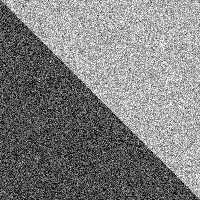
\includegraphics[width=6cm]{pictures/BW/noisy_reference.png}
    \caption{Dummy image with and without noise for edge-aware smoothing}
    \label{fig:dummy}
\end{figure}

The default filter parameters are $\lambda = 100$, $\sigma_xy = 10$ and $\sigma_l = 50$. For each parameter, deviations around these standard settings are tested and commented.

\medskip

First, the influence of the regularization parameter $\lambda$ is studied in figure \ref{fig:lambda}. For small values of $\lambda$, the regularization term doesn't have any effect, and the target image is simply copied. As $\lambda$ grows larger, the regularization kicks in, but when it gets too large the target image becomes forgotten and all that matters is regularity, leading to a uniform result.

\begin{figure}
    \centering
    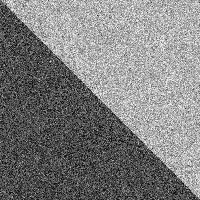
\includegraphics[width=3.5cm]{pictures/BW/smoothing_diag_lambda_1_10_50_new.png}
    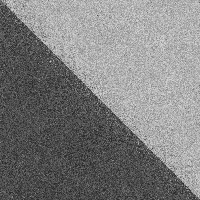
\includegraphics[width=3.5cm]{pictures/BW/smoothing_diag_lambda_10_10_50_new.png}
    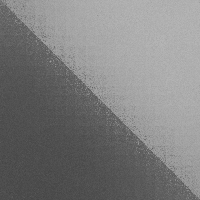
\includegraphics[width=3.5cm]{pictures/BW/smoothing_diag_lambda_100_10_50_new.png}
    
\includegraphics[width=3.5cm]{pictures/BW/smoothing_diag_lambda_1000_10_50_new.png}
    \caption{Result of the edge-aware smoothing with $\lambda = 1, 10, 100, 1000$}
    \label{fig:lambda}
\end{figure}

\medskip

Then, the influence of the spatial filter radius $\sigma_{xy}$ is analyzed in figure \ref{fig:sigma_xy}. For small values of $\sigma_{xy}$, the spatial smoothing is limited, allowing several outliers to exist when they should have been averaged with their neighbors. As $\sigma_{xy}$ grows larger, the interior of the regions becomes smoother but square artefacts appear. They are the result of the hard nearest-neighbor assignment: the groups of pixels whose associated vertices have the same spatial coordinates are large, and the transition between them is sudden.

\begin{figure}
    \centering
    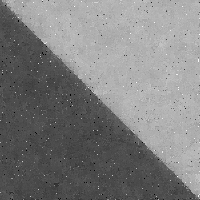
\includegraphics[width=3.5cm]{pictures/BW/smoothing_diag_sigmaxy_100_2_50_new.png}
    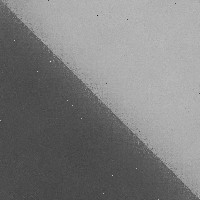
\includegraphics[width=3.5cm]{pictures/BW/smoothing_diag_sigmaxy_100_5_50_new.png}
    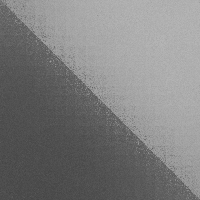
\includegraphics[width=3.5cm]{pictures/BW/smoothing_diag_sigmaxy_100_10_50_new.png}
    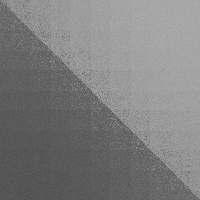
\includegraphics[width=3.5cm]{pictures/BW/smoothing_diag_sigmaxy_100_20_50_new.png}
    \caption{Result of the edge-aware smoothing with $\sigma_{xy} = 2, 5, 10, 20$}
    \label{fig:sigma_xy}
\end{figure}

\medskip

Finally, the influence of the luminance filter radius $\sigma_{l}$ is demonstrated in figure \ref{fig:sigma_l}. For small values of $\sigma_l$, the filter is very edge-aware (but not very meaningful since the default value of $\sigma_{xy}$ is also quite small). As $\sigma_l$ grows larger, the nearest-neighbor assignment is more and more controlled by the spatial filter radius $\sigma_{xy}$, which means the artefacts reappear, and the edge becomes less sharp.

\begin{figure}
    \centering
    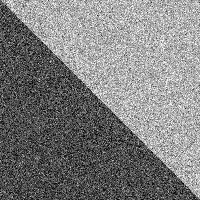
\includegraphics[width=3.5cm]{pictures/BW/smoothing_diag_sigmal_100_10_5_new.png}
    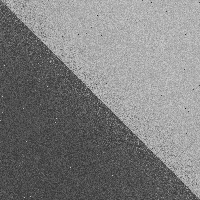
\includegraphics[width=3.5cm]{pictures/BW/smoothing_diag_sigmal_100_10_20_new.png}
    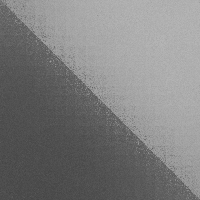
\includegraphics[width=3.5cm]{pictures/BW/smoothing_diag_sigmal_100_10_50_new.png}
    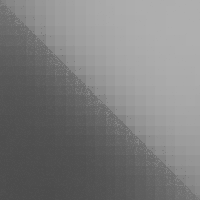
\includegraphics[width=3.5cm]{pictures/BW/smoothing_diag_sigmal_100_10_200_new.png}
    \caption{Result of the edge-aware smoothing with $\sigma_{l} = 5, 20, 50, 200$}
    \label{fig:sigma_l}
\end{figure}

\subsubsection{Cartooning and sharpening}

Besides analyzing the behaviour of the algorithm, there are other applications to edge-aware smoothing. Even when there is no need for denoising, it can be used to give images a cartoon aspect, or sharpen their details.

\medskip

Here is an example of cartooning and sharpening applied to a landscape photograph (see figure \ref{fig:auvergne_original}) taken in one of France's most beautiful places: the Auvergne region \footnote{Picture taken from \texttt{https://www.pleinevie.fr/loisirs/tourisme/france/volcans-d-auvergne\\-cap-sur-des-puys-a-la-chaine-21316}}. The algorithm parameters were $\lambda = 100$, $\sigma_{xy} = 10$, $\sigma_{rgb} = 50$ (judging by the final result, no domain transform post-processing was necessary).

Figure \ref{fig:auvergne} presents the results of smoothing, and then the superposition of the original image $I$ and the difference between $I$ and its smoothed version $S(I)$: $I + [S(I) - I]$ is an image where the details of the original are more prevalent.

\begin{figure}
    \centering
    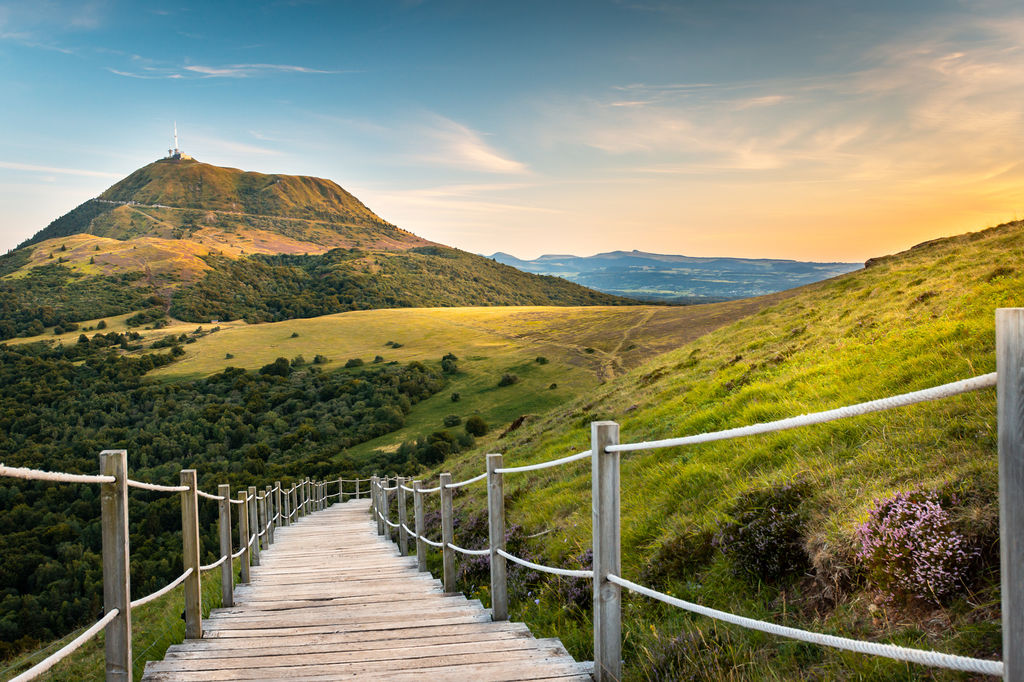
\includegraphics[width=7cm]{pictures/smoothing_auvergne_ref.png}
    \caption{Original picture taken from the Puy de Pariou}
    \label{fig:auvergne_original}
\end{figure}

\begin{figure}
    \centering
    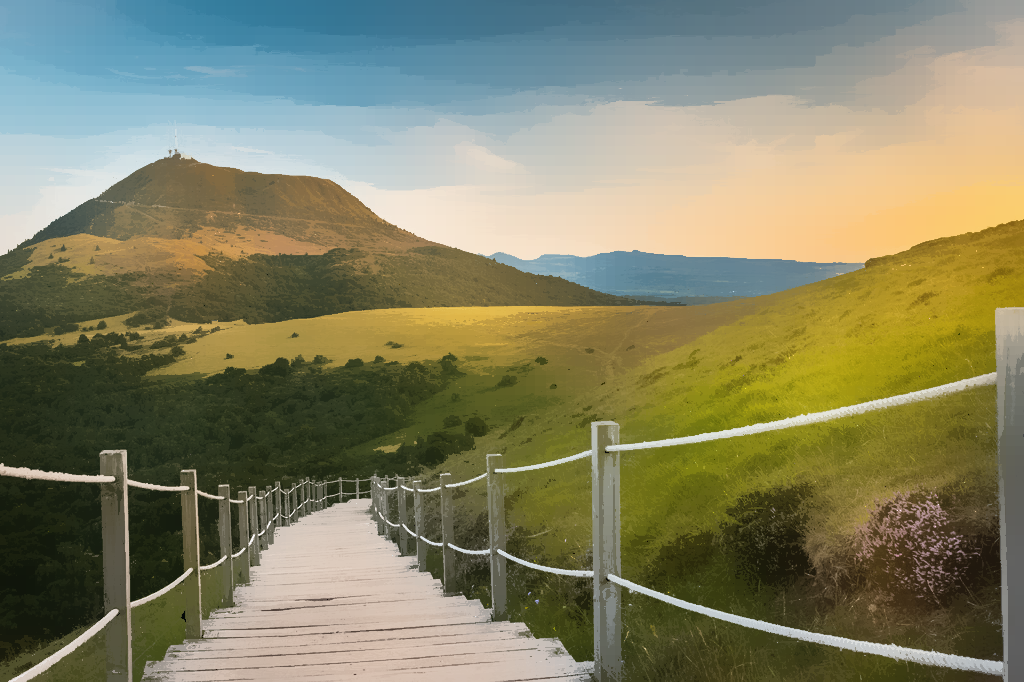
\includegraphics[width=7cm]{pictures/smoothing_auvergne_new.png}
    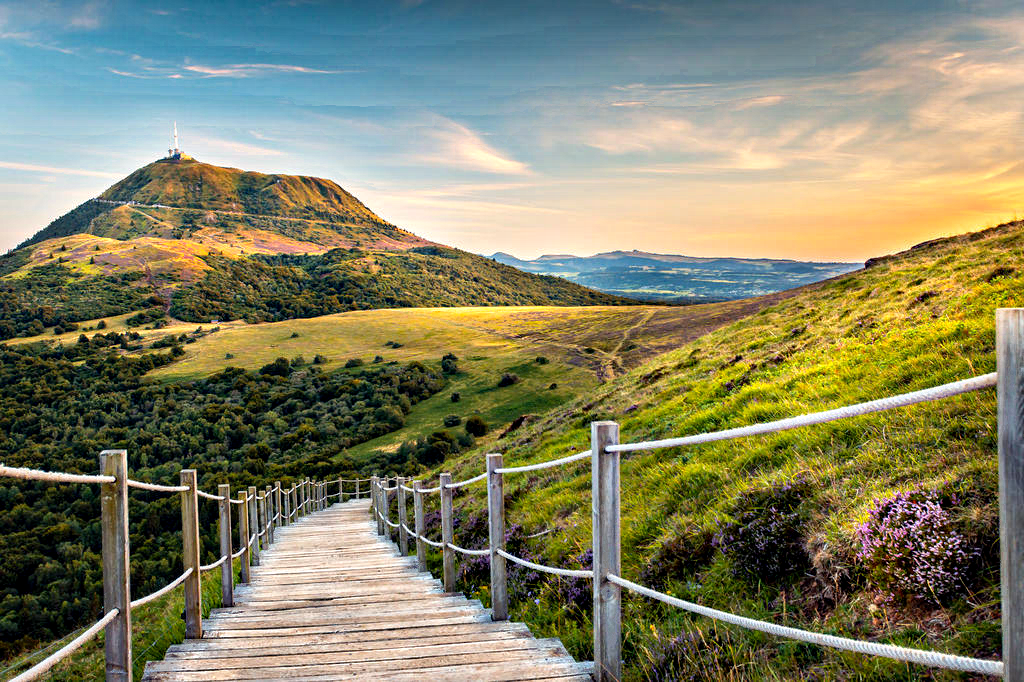
\includegraphics[width=7cm]{pictures/smoothing_auvergne_sharp.png}
    \caption{Result of edge-aware smoothing and subsequent sharpening}
    \label{fig:auvergne}
\end{figure}

\subsubsection{Depth superresolution}

Another use of the Fast Bilateral Solver is the improvement of low quality depth maps with the help of a color image. While color images taken by standard cameras often have little noise and high resolution, depth maps can be very noisy and have a much lower resolution.

The algorithm we present enables us to improve the depth map by drawing inspiration from the structure of the reference color image.

\medskip

Approximately following the test procedure laid out by \cite{ferstl_image_2013}, we start with a pair (image, disparity map) taken from the Middlebury dataset \cite{jiang_high-resolution_2014}. From the disparity map we deduce a depth map, which is then downsampled by a factor of $f=8$, combined with a Gaussian noise (whose variance is proportional to the local disparity) and eventually reupsampled using interpolation. These two starting points are displayed in figure \ref{fig:room_original}.

\begin{figure}
    \centering
    \includegraphics[width=9cm]{pictures/depth_superresolution_room_ref.png}
    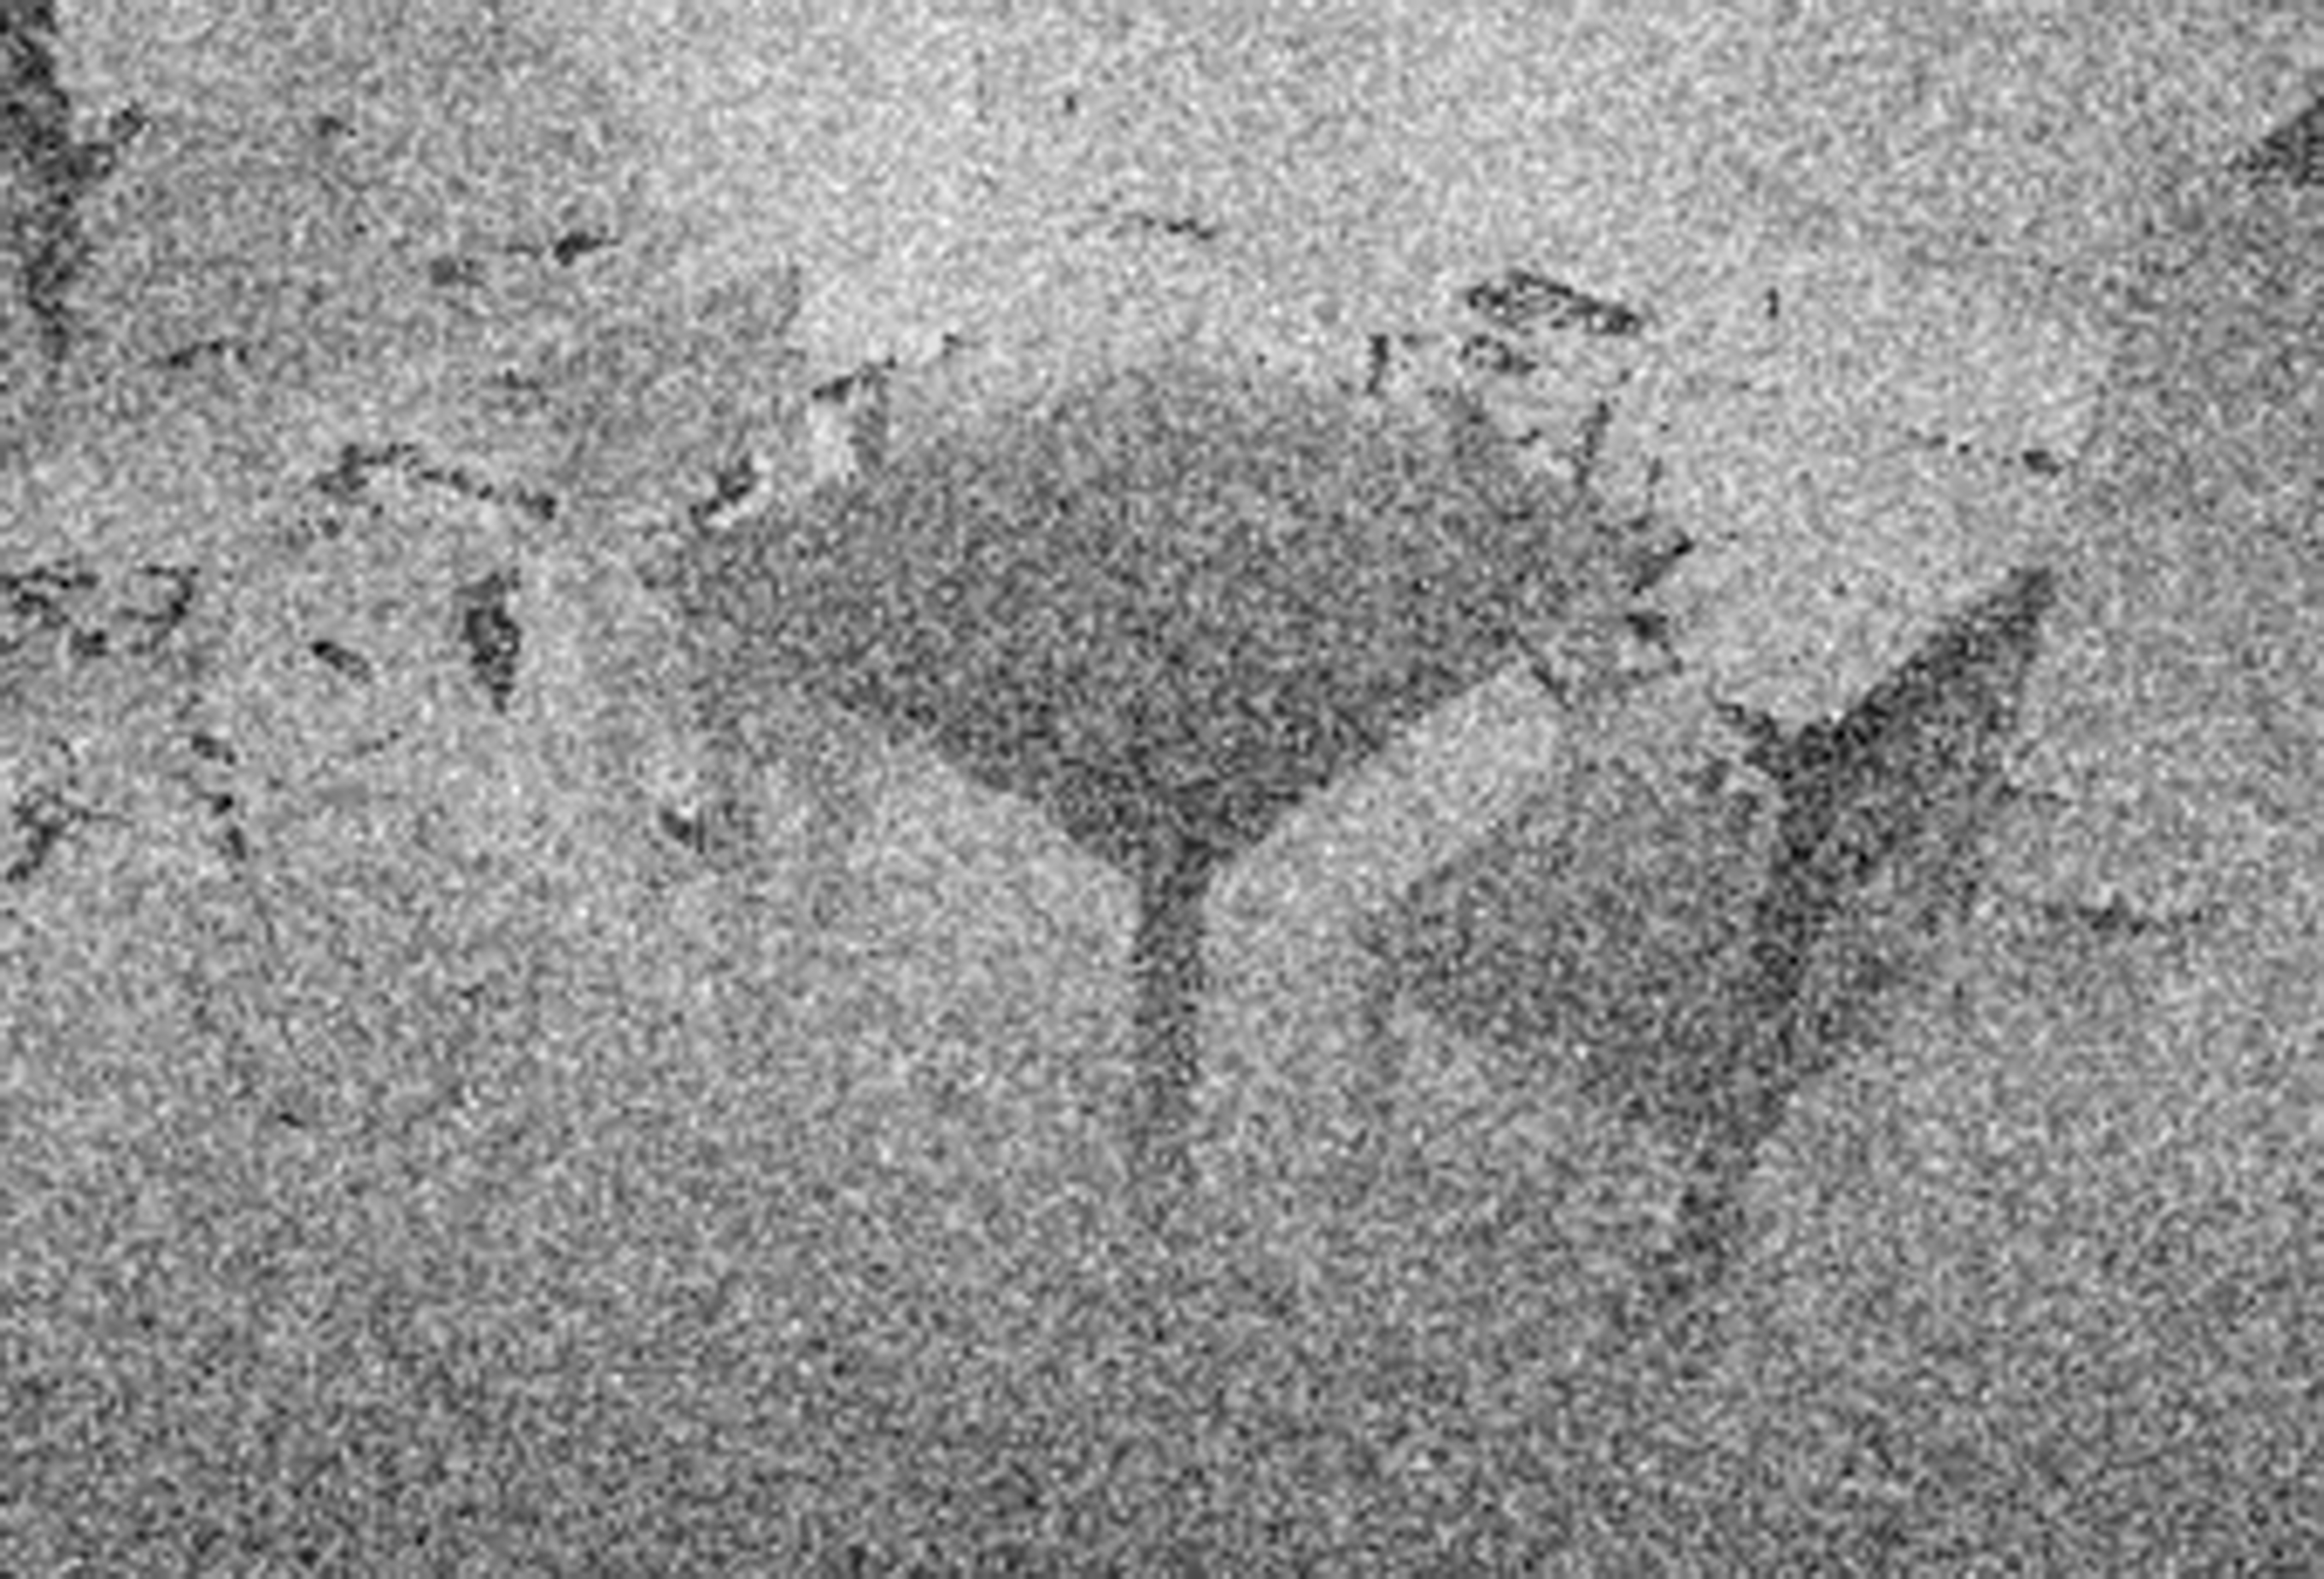
\includegraphics[width=5cm]{pictures/depth_superresolution_room_target.png}
    \caption{High-resolution color reference and noisy low-resolution depth map}
    \label{fig:room_original}
\end{figure}

\medskip

The result of the procedure can be observed in figure \ref{fig:room}. While it is globally convincing, some things are still not right. Regarding the "cloudy" aspect, it is probably caused by the high amplitude of the Gaussian noise, leading to irregularities even in the supposedly uniform regions.

However, the fact that the supposed depth of the chess board (left-hand side of the scene) varies so wildly is much more problematic. This is due to the denoising procedure working from a color image, and trying to abide by its edges. While the edges of the chess squares are indeed very sharp in the color reference, they do not correspond to limits between objects on separate depth levels. This causes errors in the depth reconstruction performed by the algorithm.

\begin{figure}
    \centering
    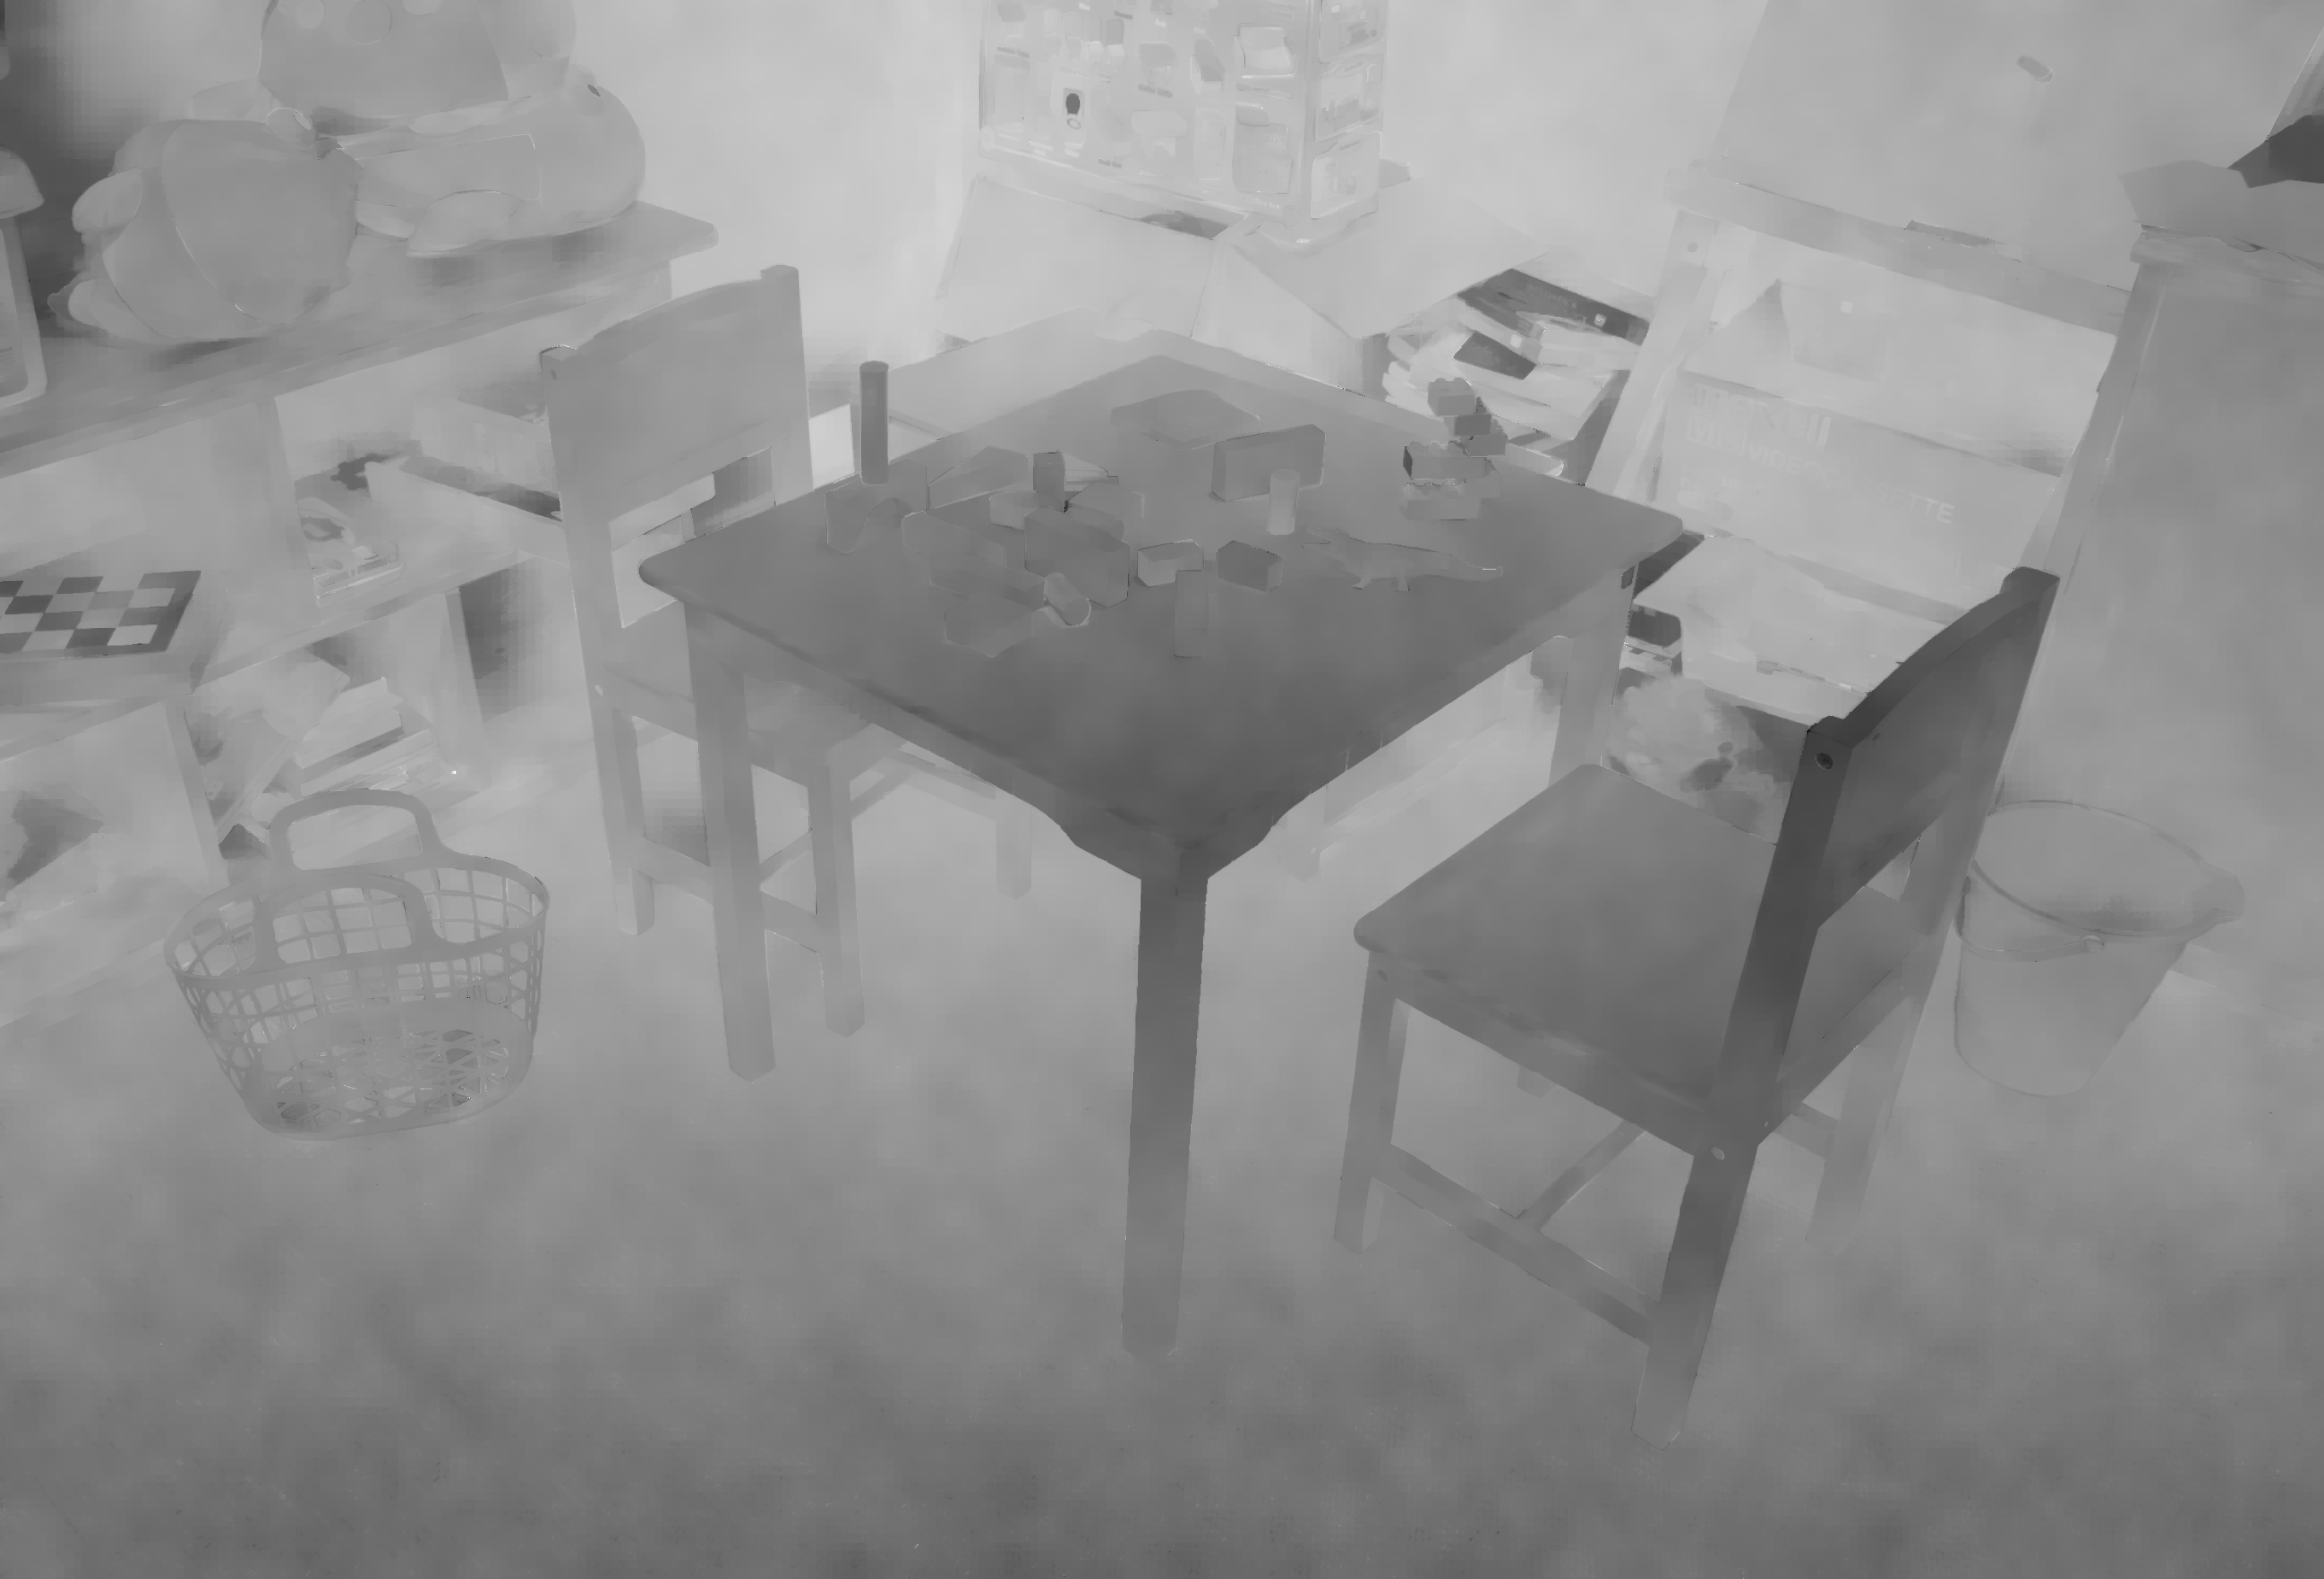
\includegraphics[width=10cm]{pictures/depth_superresolution_room_new.png}
    \caption{High-resolution denoised depth map}
    \label{fig:room}
\end{figure}

\subsubsection{Colorization}

Finally, as mentioned in the beginning of this report, the Fast Bilateral Solver works very well for colorization. The target image is a black and white picture color-marked by the user in certain areas where the color is (approximately known). The algorithm's purpose is then to expand and conciliate these color stains, while respecting the structure of the reference black and white image.

\medskip

We worked on a black and white picture of the Hindenburg's crash in 1937, taken by Murray Becker. The color markings were done in a very rough way, aiming at an esthetically pleasing result rather than a historically correct one: they are reproduced in figure \ref{fig:hindenburg_original}.

As for the algorithm parameters, we used the following settings: $\lambda = 5$, $\sigma_{xy} = 10$, $\sigma_l = 40$, $\sigma_{xy}' = 2$, $\sigma_{luv}' = 20$. 

\medskip

The colorized result can be seen in figure \ref{fig:hindenburg}. We notice that the color blue has spread across the whole night sky, changing its shade according to the luminance structure of the black and white reference. The yellow and red colors have extended their areas too, but always stopping at sharp edges of the original image (e.g. the limits of the aircraft or the smoke cloud).

\begin{figure}
    \centering
    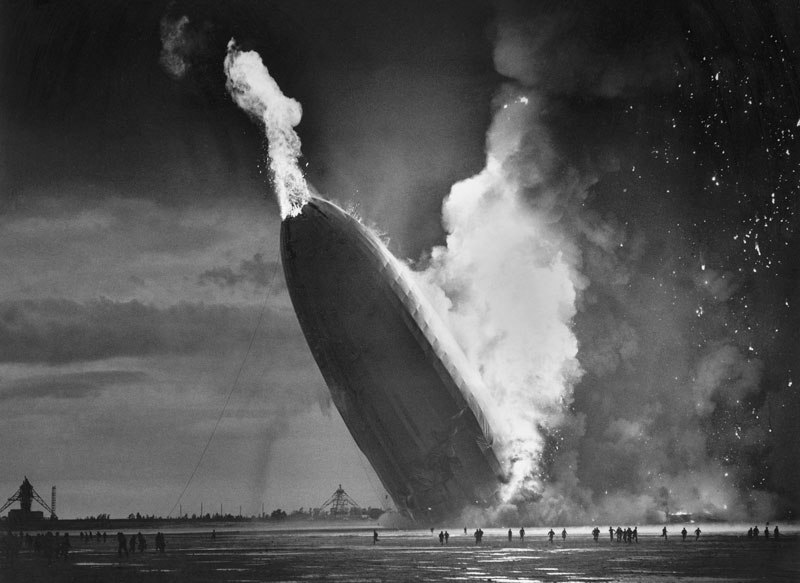
\includegraphics[width=7cm]{pictures/colorization_hindenburg_ref.png}
    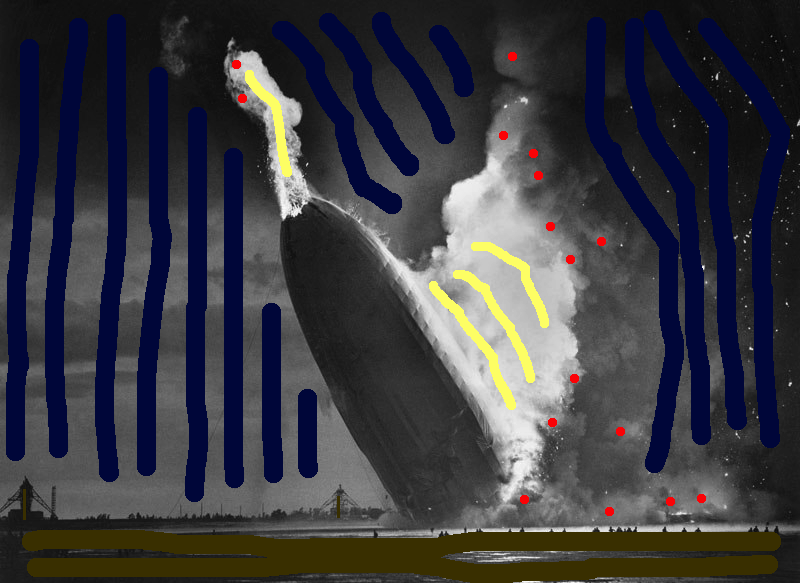
\includegraphics[width=7cm]{pictures/colorization_hindenburg_target.png}
    \caption{Black \& white original and color-marked versions of the Hindenburg disaster}
    \label{fig:hindenburg_original}
\end{figure}

\begin{figure}
    \centering
    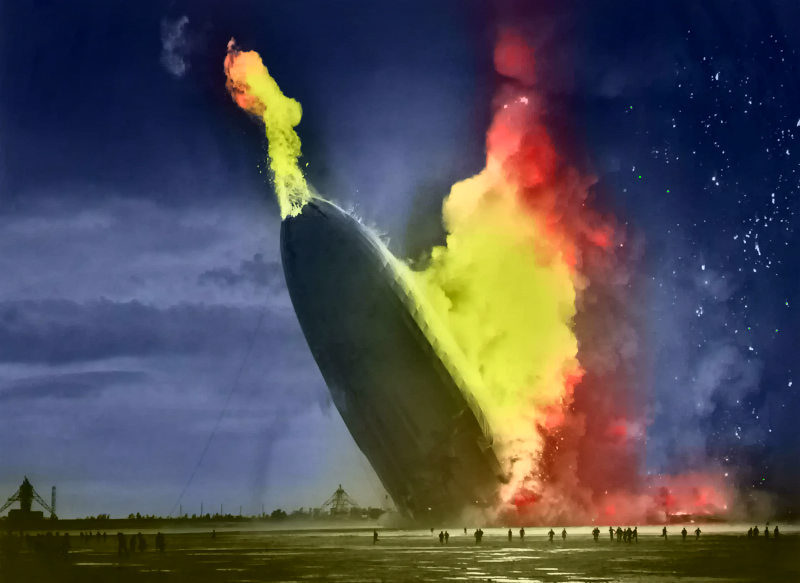
\includegraphics[width=13cm]{pictures/colorization_hindenburg_new.png}
    \caption{Automatically colorized version of the Hindenburg disaster}
    \label{fig:hindenburg}
\end{figure}

\subsection{Discussion}

\subsubsection{Advantages}

The Fast Bilateral Solver presents several advantages over previous methods, which make it interesting in a number of situations. Here are a few:

\begin{itemize}
    \item As its name suggests, it is very fast. Compared to other baseline techniques on several applications (including those mentioned above), its runtime is diminished significantly without compromising the accuracy.
    
    On the one hand, using the simplified bilateral grid makes the computation of the splat-blur-slice decomposition $W \simeq S^T B S$ near instantaneous even for large images. On the other hand, the bilateral space in which we work has a very low dimension compared to the original pixel space. Finally, the formulation of the problem as a least-squares optimization allows the use of very efficient minimization routines such as the conjugate gradient descent, further optimized by a hierarchical preconditioner.
    
    \item For the same reasons of dimensionality reduction, this algorithm requires low memory.
    
    \item It is rapidly implementable in any programming language: the only crucial requirement is an efficient implementation of sparse matrices.
    
    \item It has few hyperparameters, all of which have a clear intuitive meaning ($\lambda$ for regularization and $\sigma$ for the filter radius) being the most important ones.
    
    \item It is general: the idea of splat-blur-slice factorization can be applied accross a whole range of image processing problems.
    
    \item It is easily integrated into a deep learning pipeline, because the backpropagation of the error on $\textbf{x}$ onto the error on $\textbf{t}, \textbf{c}$ can be written explicitly.
    
\end{itemize}

\subsubsection{Possible improvements}

However, some drawbacks still make this procedure perfectible. Moreover, some parts in the article were not very clear, or deserve improvements. We will try to list a few shortcomings below:

\begin{itemize}
    \item The complexity of the algorithm is dependent upon the value of the filter radius $\sigma$. The smaller the values in $\sigma$, the more bilateral vertices there will be, which slows down the whole procedure.
    
    \item The simplified bilateral grid, while easy to implement, comes with caveats. The hard nearest-neighbor assignment causes square artefacts which must be removed through post-processing or smaller values of $\sigma_{xy}$.
    
    This can be solved through the use of more sophisticated grids, such as the permutohedral lattice of \cite{adams_fast_2010}, which splats a pixel onto several vertices. However, the implementation becomes substantially more complicated as a result, and the runtime of the algorithm increases due to harder nearest-neighbor computations and a less sparse $S$ matrix.
    
    \item The frequent use of domain transform post-processing in the article makes it hard to separate between the merits of both procedures, which were both designed to solve the same problem. While in a few settings, we indeed observed that the domain transform allowed for a reduction of the square artefacts induced by the simplified bilateral grid, maybe changing the parameters of the grid would have helped as well. If the domain transform is always necessary, it may mean the initial algorithm is not sufficient.
    
    In addition, although our \textsc{Python} code was heavily profiled and optimized, the domain transform remained (by far) the slowest part of the procedure, which is why (most of the time) we dispensed with it to focus on the Fast Bilateral Solver per se.
\end{itemize}

\newpage

\bibliographystyle{plain}
\bibliography{sources}

\end{document}

